\begin{pastexam}[label={px:nsysu-114-osds-03}]{中山資工所甲組 114 學年度 第 3 題}
（追蹤）

The following figure is an AVL tree.
\begin{enumerate}[label=(\alph*)]
\item (5\%) Draw the AVL tree after a new element 1 is inserted.
\item (5\%) Draw the AVL tree after a new element 4 is inserted (1 is not inserted).
\end{enumerate}
\begin{center}
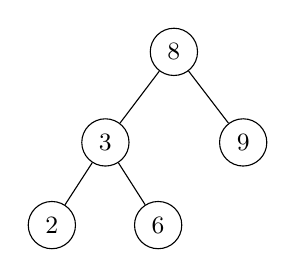
\begin{tikzpicture}[v/.style={circle,draw,minimum size=6mm,inner sep=0pt,font=\small}]
\node[v] (8) at (5.17,-18.73) {8};
\node[v] (3) at (4.30,-19.88) {3};
\node[v] (9) at (6.05,-19.88) {9};
\node[v] (2) at (3.62,-20.93) {2};
\node[v] (6) at (4.97,-20.93) {6};
\draw (8) -- (3);
\draw (8) -- (9);
\draw (3) -- (2);
\draw (3) -- (6);
\end{tikzpicture}
\end{center}
\end{pastexam}

\begin{pastsoln}
答案：(a) 根 $3$，左 $2(1, -)$，右 $8(6, 9)$；(b) 根 $6$，左 $3(2, 4)$，右 $8(-, 9)$。 圖在下面。

做法照資結書第~10.2.3~節：先照二元搜尋樹插入，再從新節點往上找第一個平衡因子變成 $\pm 2$ 的節點，依新節點在它
的哪一邊（LL、LR、RL、RR）旋轉。 平衡因子 $= $ 左子樹高度 $-$ 右子樹高度。 原樹中 $8$ 的平衡因子是 $+1$（左高
$2$、右高 $1$），其他節點都是 $0$。

\textbf{(a) 插入 $1$。} $1 < 8$、$1 < 3$、$1 < 2$，放在 $2$ 的左邊。 往上：$2$ 變 $+1$，$3$ 變 $+1$，$8$ 的左子樹高度
變 $3$、右子樹 $1$，平衡因子 $+2$，失衡。 新節點在 $8$ 的左子節點 $3$ 的\textbf{左}子樹，是 LL 型：對 $8$ 做一次右旋。
$3$ 升為根，$8$ 成為 $3$ 的右子節點，$3$ 原來的右子樹 $6$ 改掛到 $8$ 的左邊。

\textbf{(b) 插入 $4$（從原樹開始）。} $4 < 8$、$4 > 3$、$4 < 6$，放在 $6$ 的左邊。 往上：$6$ 變 $+1$，$3$ 變 $-1$，$8$
變 $+2$，失衡。 新節點在 $8$ 的左子節點 $3$ 的\textbf{右}子樹，是 LR 型：先對 $3$ 左旋、再對 $8$ 右旋（雙旋轉），
結果是 $3$、$8$ 之間的 $6$ 升為根。 $6$ 原來的左子樹 $4$ 掛到 $3$ 的右邊，$6$ 原來的右子樹（空的）掛到 $8$ 的左邊。

\begin{center}
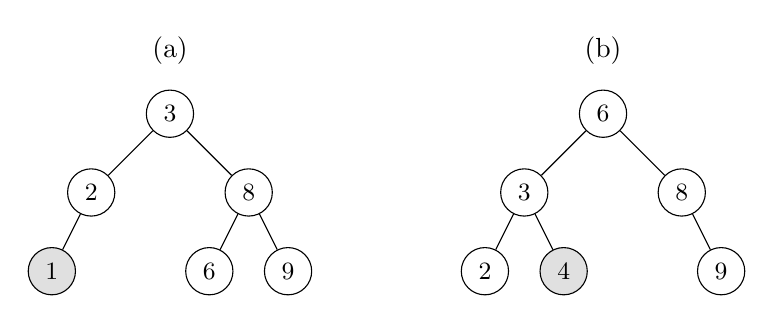
\begin{tikzpicture}[v/.style={circle,draw,minimum size=6mm,inner sep=0pt,font=\small},
  nv/.style={v,fill=black!12},
  level distance=10mm, level 1/.style={sibling distance=20mm}, level 2/.style={sibling distance=10mm}]
\node at (0,0.8) {(a)};
\node[v] at (0,0) {3}
  child {node[v] {2} child {node[nv] {1}} child[missing]}
  child {node[v] {8} child {node[v] {6}} child {node[v] {9}}};
\begin{scope}[xshift=55mm]
\node at (0,0.8) {(b)};
\node[v] at (0,0) {6}
  child {node[v] {3} child {node[v] {2}} child {node[nv] {4}}}
  child {node[v] {8} child[missing] child {node[v] {9}}};
\end{scope}
\end{tikzpicture}
\end{center}
（灰色是新插入的節點。） 檢查：(a) 中序是 $1, 2, 3, 6, 8, 9$，仍是二元搜尋樹；平衡因子 $3$ 是 $0$（左右子樹高度都是
$2$），$2$ 是 $+1$，其餘是 $0$。 (b) 中序是 $2, 3, 4, 6, 8, 9$；平衡因子 $6$ 是 $0$、$3$ 是 $0$、$8$ 是 $-1$，其餘是 $0$。
兩棵都是合法的 AVL 樹。
\end{pastsoln}
